\documentclass[12pt]{article}

\usepackage{amsmath}
\usepackage{graphicx}
\usepackage{enumerate}
\usepackage{natbib}
\usepackage{url} % not crucial - just used below for the URL 
\usepackage{color}
 \usepackage{multirow}
\newcommand{\todo}[1]{{\color{red}{TO DO: \sc #1}}}

%\pdfminorversion=4
% NOTE: To produce blinded version, replace "0" with "1" below.
\newcommand{\blind}{0}

% DON'T change margins - should be 1 inch all around.
\addtolength{\oddsidemargin}{-.5in}%
\addtolength{\evensidemargin}{-.5in}%
\addtolength{\textwidth}{1in}%
\addtolength{\textheight}{1.3in}%
\addtolength{\topmargin}{-.8in}%


\begin{document}

%\bibliographystyle{natbib}

\def\spacingset#1{\renewcommand{\baselinestretch}%
{#1}\small\normalsize} \spacingset{1}


%%%%%%%%%%%%%%%%%%%%%%%%%%%%%%%%%%%%%%%%%%%%%%%%%%%%%%%%%%%%%%%%%%%%%%%%%%%%%%

\if0\blind
{
  \title{\bf A Comparison of Parametric and Permutation Tests for Regression Analysis of Randomized Control Trials}
\author{Kellie Ottoboni \\
Department of Statistics; Berkeley Institute for Data Science\\
University of California, Berkeley \\ 
Fraser Lewis \\
RB\\ 
Luigi Salmaso\\
Department of Management and Engineering \\
University of Padova
}  \maketitle
} \fi

\if1\blind
{
  \bigskip
  \bigskip
  \bigskip
  \begin{center}
    {\LARGE\bf  A Comparison of Parametric and Permutation Tests for Regression Analysis of Randomized Control Trials}
\end{center}
  \medskip
} \fi

\bigskip
\begin{abstract}
% 200 words or less
Hypothesis tests based on the linear model are widely accepted by organizations that regulate clinical trials.
We focus on analysis of covariance (ANCOVA), a special case of linear regression that incorporates stratification.
ANCOVA is derived using strong assumptions about the data-generating process so that the resulting inference is based on parametric distributions.
Because these methods are well understood and robust, they are sometimes applied to data that depart from assumptions, such as ordinal integer scores.
Permutation tests are a nonparametric alternative that require minimal assumptions which are often guaranteed by the randomization that was conducted.
We compare ANCOVA to several permutation tests based on linear models that control for pretreatment covariates.
In simulated trials using a variety of data-generating processes, some of which violate the parametric assumptions,
the permutation tests maintain power comparable to the ANCOVA.
We illustrate the use of these permutation tests alongside ANCOVA with data from a clinical trial comparing the effectiveness of two treatments for gastroesophageal reflux disease.
Given the considerable costs and scientific importance of clinical trials, one may want to include an additional robust method, such as a linear model permutation test, as a check on the statistical inference for the main study endpoints.
\end{abstract}

\noindent%
{\it Keywords:}  nonparametric, linear model, ANCOVA, inference
\vfill

\newpage
%\spacingset{1.45} % DON'T change the spacing!
\section{Background}
A hypothesis test is a statistical method for determining whether observed data is consistent with a belief about the process that generated the data.
Medical experiments use hypothesis testing to assess the evidence that a treatment affects one or more clinically relevant outcomes.
The simplest version of this experiment, which involves randomly assigning two treatments to a fixed number of individuals in a group and measuring a single outcome, has been studied for nearly a century (see \cite{fisher_design_1935} and \cite{neyman_application_1923} for early references).
One can conduct hypothesis tests and construct confidence intervals for the estimated treatment effect
by exploiting the fact that the difference in average outcomes between the two treatment groups is asymptotically normal with a variance that can be estimated from the data.

Randomized experiments in the real world are rarely this simple:
if individuals are heterogeneous before the study, then their outcomes may differ for reasons besides the treatment;
there may be more than two treatments under study;
patients may not take the treatment they are assigned or may drop out of the study;
and an individual's assignment to treatment may affect others' outcomes.
Techniques have been developed to deal with each of these issues, invoking additional assumptions in order to carry out valid inference.
%For any particular dataset, it is difficult to determine to what extent the assumptions for asymptotic normality are satisfied.
In this paper, we focus on the issue of heterogeneity of pretreatment characteristics and assume that the other issues are not present.

Random assignment of treatment ensures that pretreatment covariates are balanced between treatment groups on average, across all possible randomizations.
However, in any particular randomization, there may be imbalances.
If the imbalanced variables are associated with the outcome, then even when treatment has no effect, there may be differences in outcomes between treatment groups.
Adjusting for such covariates can reduce the variability of treatment effect estimates and yield more powerful hypothesis tests.

Stratification is one method to control for covariates that are known a priori to be associated with the outcome.
Strata are groups of individuals with similar levels of a covariate, and random assignment of treatments is conducted within each group, independently across groups.
The stratification is done \textit{before any outcome data is collected}.
This guarantees that the stratification variable is balanced between treatment groups.
A common stratification variable in clinical experiments is location:
individuals often come from many sites because it is difficult to recruit a sufficient number of participants at one doctor's office or hospital,
especially when the object of study is a rare disease or a rare outcome.
Controlling for stratum can have the same beneficial effects as controlling for other pretreatment covariates, 
as outcomes may vary across strata due to factors unrelated to individuals.

Linear regression is another way to control for baseline covariates.
It is done \textit{after} data are collected and outcomes have been observed.
While stratification guarantees balance on the stratifying variable, other covariates may still be imbalanced.
Stronger modeling assumptions may be necessary to balance them after the fact.
Linear regression is a method which projects the outcomes onto the plane that best summarizes each variable's relationship to the outcome.
The coefficient of any particular covariate answers the question, if we were to hold fixed all other variables and increase this variable by one unit, how much would we expect the outcome to change?
This model posits a linear relationship between covariates, treatment, and outcome; 
if the true relationship is not linear, then linear regression gives the best linear approximation to the conditional expectation of the outcome.
When controlling for strata, such as location, it is standard to use analysis of covariance (ANCOVA).
ANCOVA is a particular version of linear regression that allows each stratum to have its own mean outcome level.
This amounts to fitting a plane to each stratum, allowing each plane to have a different intercept but requiring them to have a common slope.

Hypothesis testing of estimated coefficients requires even stronger assumptions than linearity, namely Gaussian, homoskedastic errors.
When this holds, a regression coefficient scaled by its estimated variance follows Student's $t$ distribution.
Thus, if we believe the linear model is correctly specified, a hypothesis test for a treatment effect amounts to a hypothesis test of the coefficient for treatment in the ANCOVA model can be evaluated analytically and quickly.
However, the modeling assumptions are clearly violated in many cases:
when the data are discrete or ordinal, 
when the treatment has a differential effect across subgroups of individuals and no interaction terms are included, 
and when measurement error sizes differ across strata.
Furthermore, the hypothesis test implicitly assumes that the data were sampled at random from some underlying population, when in fact,
medical experimenters rarely recruit patients this way (\cite{ludbrook_why_1998}).

Permutation testing is an alternate approach (\cite{fisher_design_1935, pitman_significance_1937,pitman_significance_1938}).
Deliberate randomization induces a distribution for any test statistic under the null hypothesis that treatment has no effect on the outcome:
the randomization scheme provides information about all possible ways that treatment may have been assigned 
and the null hypothesis tells us what each individual's response would be regardless of the assignment (namely, it would be the same).
One determines how ``extreme'' the observed test statistic is relative to this randomization distribution, rather than a parametric reference distribution like Student's $t$ or the standard Gaussian.
Such a test is exact, meaning that it controls the type I error rate at the pre-specified level even in finite samples, whereas parametric hypothesis tests based on asymptotic approximations do not always guarantee good finite sample properties.
Permutation tests achieve this by operating conditional on the observed sample; the resulting inference applies to the sample at hand, but does not necessarily generalize to other groups of individuals.
This may be acceptable when the individuals who make up the sample are not representative of any well-defined population.

In the past, parametric tests were necessary because asymptotic approximations were the only computationally feasible way to estimate distributions. 
Now, computational power is no longer a barrier to finding exact (or exact to pre-specified precision) randomization distributions.
In most cases, a randomization test is the ``gold standard'':
``[a] corresponding parametric test is valid only to the extent that it results in the same statistical decision [as the randomization test]'' (\cite{bradley_distribution_1968}).
Therefore, when conducting creating estimates and confidence intervals using parametric methods, one may have greater confidence in the results when the decision to accept or reject the null hypothesis is the same for the parametric and permutation tests.

There is no hard and fast rule describing the rate at which parametric tests approach the exact permutation solution, as they are both highly dependent on the particular data observed.
On the one hand, some argue that violations of parametric test assumptions necessitate the use of permutation methods.
\cite{ludbrook_why_1998} point out that medical trials rarely follow the population sampling model implicit in parametric methods.
Many people recommend using permutation tests in place of the usual parametric tests for typical analyses, such as ANOVA and generalized linear models (\cite{still_approximate_1981, winkler_permutation_2014}).
They argue that there are a myriad of ways that the data may violate the necessary assumptions for the test, and so it is more robust to use a permutation test.

However, parametric and nonparametric tests seem to perform similarly when compared side-by-side in simulations, even when data violate the assumptions of the parametric method.
Medical trials studying pain or perceived severity scores often use Likert scale data, which is discrete and does not match the normality assumptions of parametric tests.
However, \cite{winter_five-point_2010} found that the two sample $t$ test and Mann-Whitney test had comparable Type I and II error rates for five-point Likert scale data, suggesting that the violation of normality does not entirely invalidate the parametric test.
\cite{vickers_parametric_2005} compared the parametric ANCOVA to the Mann-Whitney rank test in the context of randomized experiments, finding that except in extreme situations, ANCOVA was more powerful than the nonparametric test.
Most similar to our question of study, \cite{anderson_empirical_1999} found little difference between several permutation tests for coefficients in a linear model alongside the parametric $t$ test.

In this paper, we review several hypothesis tests for a treatment effect which adjust for pretreatment covariates to increase power.  
We focus on ANCOVA and its permutation counterparts, comparing their performance in different scenarios and illustrating their application with a clinical dataset.
We find in simulations that even when assumptions are not satisfied, the parametric and permutation tests have comparable power to detect a treatment effect.
We apply each of the methods to data from a clinical trial which assessed the performance of two treatments for gastroesophageal reflux disease (GERD).
We conclude by discussing implications of these results for practitioners.

\section{Methods}
% The methods section should include:

%the aim, design and setting of the study
%the characteristics of participants or description of materials
%a clear description of all processes, interventions and comparisons. Generic drug names should generally be used. When proprietary brands are used in research, include the brand names in parentheses
%the type of statistical analysis used, including a power calculation if appropriate

\subsection{Notation}
Suppose we randomly assign two treatments labelled $0$ and $1$ to a group of individuals.
We are interested in comparing the relative effectiveness of treatment 1 to treatment 0.
Let $\mathbf{Z}$ indicate treatment assignment, 0 or 1, 
$\mathbf{Y}$ denote the observed outcome of interest,
and $\mathbf{X}$ be a pretreatment covariate that is observed and associated with the outcome.
For expository clarity, we suppose that $\mathbf{X}$ is univariate, but all results are easily extended to the case when $\mathbf{X}$ is multivariate.
Suppose further that there is a categorical pretreatment variable with $J$ levels used to stratify individuals. 

We observe $\{Y_{ij}, Z_{ij}, X_{ij}\}$ for individuals $i = 1, \dots, n_j$, in strata $j = 1, \dots, J$.
All individuals have two potential outcomes, $Y_{ij}(1)$ and $Y_{ij}(0)$, representing their responses to treatments $1$ and $0$, respectively.
We can never observe both; random assignment of treatment reveals $Y_{ij} = Z_{ij}Y_{ij}(1) + (1-Z_{ij})Y_{ij}(0)$.
Throughout, we assume that there is no interference between individuals 
(in other words, $Y_{ij}$ is a function of $(Z_{ij}, Y_{ij}(1), Y_{ij}(0))$ and not any other $Z_{i', j'}$)
and that there is no non-compliance or study dropout 
(we actually observe $Y_{ij} = Y_{ij}(Z_{ij})$ for all $i, j$).

We are interested in the differences in potential outcomes $Y_{ij}(1) - Y_{ij}(0)$.
This quantity represents the effect of treatment for individual $i$ in group $j$: 
it is the difference between what we would have observed under treatment 1 and what we would have observed under treatment $0$.
A typical problem is to estimate the average of differences $Y_{ij}(1) - Y_{ij}(0)$ in some group, such as the study sample or in a target population.
Which function of these differences will be considered depends on the chosen method of analysis.
Any of these possible quantities may be of clinical interest; it is a matter of philosophy which one prefers.
Rather than estimation, we will focus on hypothesis testing for whether these differences are nonzero.

\subsection{Parametric ANCOVA}

The model is

\begin{equation}\label{eqn:ancova}
Y_{ij} = \alpha_j + \beta X_{ij} + \gamma Z_{ij} + \varepsilon_{ij}
\end{equation}

\noindent where $\alpha_j$ is a fixed effect for stratum $j$, $\beta$ is the coefficient for the pretreatment covariate,
$\gamma$ is the coefficient for treatment,
and $\varepsilon_{ij}$ is an error term.
The parameter of interest is $\gamma$. 
If we believe the linear model is the true data-generating process, it asserts that for each individual, $Y(1) = Y(0) + \gamma$.
However, we needn't take this perspective for $\gamma$ to be a useful quantity; it represents the average treatment effect, holding the other variables fixed.
We would like to test the null hypothesis $H_0: \gamma = 0$ against
the two-sided alternative hypothesis $H_1: \gamma \neq 0$.

To carry out the standard parametric hypothesis test, we make the following assumptions (\cite{freedman_statistical_2005}):

\begin{enumerate}
\item \textbf{Linearity:} The data $\mathbf{Y}$ are related to $\mathbf{X}$ and $\mathbf{Z}$ linearly.
\item \textbf{Constant slopes:} Stratum only affects the intercept $\alpha_j$, not the slopes $\beta$ and $\gamma$.
\item \textbf{IID Errors:} The $\varepsilon_{ij}$ are independent and identically distributed with mean $0$ and variance $\sigma^2$.
\item \textbf{Independence:} If $\mathbf{X}$ is random, $\mathbf{\varepsilon}$ is statistically independent of $\mathbf{X}$.
\item \textbf{Normality:} The errors are normally distributed.
\end{enumerate}

The coefficients are estimated using least squares.
(Note, only Assumptions (1) and (2) are needed to guarantee the existence of a solution.
The solution will be unique as long as there is no linear relationship between $\mathbf{X}$, $\mathbf{Z}$, and stratum membership.)
This procedure yields an estimate of $\hat{\sigma}_{\hat{\gamma}}^2$, the  standard error of $\hat{\gamma}$
(namely, the diagonal element corresponding to the treatment variable in the inverse covariance matrix of regression covariates).
Under the null hypothesis, the test statistic 
$$ T = \frac{\hat{\gamma}}{\sqrt{ \hat{\sigma}_{\hat{\gamma}}^2}}$$
follows the Student $t$ distribution with degrees of freedom equal to the number of observations minus the number of parameters estimated (in this case, $N - J - 2$).
The $p$-value for this hypothesis test is the probability that a value drawn from the $t$ distribution is larger in magnitude than $T$.


The ANCOVA model allows for fixed stratum effects that are additive in the outcome.  
The model does not account for variation in the treatment effect across strata.  
The estimated linear model may not accurately capture details of the true data-generating process:
if effects are not constant across strata, then the coefficient $\gamma$ may be attenuated towards 0.  
A test of the null hypothesis that $\gamma = 0$ will be valid, but will not reflect the true magnitude of treatment effects among individuals.

\subsection{Stratified permutation test}
Suppose we wish to test the null hypothesis that individual by individual, treatment has no effect.
This is referred to as the ``sharp'' null hypothesis:

$$H_0: Y_{ij}(1) = Y_{ij}(0), \forall i = 1, \dots, n_j, j = 1,\dots, J.$$

Then, which treatment an individual received amounts to an arbitrary label.
Once we observe one response under a particular treatment, we can impute the other potential outcome; namely, it would have been the same.
This null hypothesis is stronger than the null hypothesis for the parametric ANCOVA, which only asserts that the treatment has no effect \textit{on average}.

For the permutation test, we condition on the number of individuals who received each treatment within each stratum.
Any assignment of treatments which preserves the number of treated units within each stratum is valid and was just as likely to occur as the randomization that was actually observed.
We can construct the permutation distribution of any statistic under the null hypothesis by using this principle of equal probabilities and imputing the unobserved potential outcomes under the sharp null hypothesis.

The most commonly used statistic is the difference in mean outcomes of people who received treatment 1 and the mean outcomes of people who received treatment 0.  
This statistic is unbiased and readily interpretable in randomized experiments (``on average, taking treatment changes the outcome by x amount''), and has nice theoretical properties owing to it being the difference of two sums.
However, the difference in means may not be optimal if we want to be sensitive to heterogeneous effects.  
For an extreme example, imagine that there an equal number of males and females in the sample, and each treatment is assigned to half of males and half of females.  
Everybody who receives treatment 0 has an outcome of 0, but males who receive treatment 1 have an outcome of $1$ and females who receive treatment 1 have an outcome of $-1$.  
Then the difference in means between the treatment groups is $0$, even though the treatment had nonzero effects on both males and females.  
This differential effect gets averaged out.

To avoid this, one may want to stratify the sample according to important confounding variables, then compute a statistic for each stratum separately. 
There is a great degree of freedom in choosing how exactly to construct such a statistic.
Two factors must be decided: how to stratify and how to combine the statistics across strata.
There is a tradeoff in how finely we choose to stratify.
On the one hand, the strata must be sufficiently large to be informative,
 but on the other hand, must be fine enough to capture variation in treatment effects.
Our simulations in Section~\ref{simulations} show a loss of power when effects are concentrated in small strata.

One way to construct a test statistic is to directly combine the statistics into a single statistic on the data, for instance taking the sum of their absolute values.
Taking the absolute value before summing ensures that effects with different signs do not cancel each other out.
The permutation test is conducted identically, using this statistic in place of the difference in means.
Another way to construct a test is to use the nonparametric combination (NPC) framework proposed by Pesarin and Salmaso \cite{pesarin_permutation_2010}.
In this framework, one would break down the ``global'' null hypothesis of no effect whatsoever into the intersection of ``partial'' null hypotheses of no treatment effect within each stratum.
For NPC, one first conducts each partial test separately, then combines their $p$-values in a way that preserves dependencies.
In this case, strata are randomized independently so there are no dependencies to preserve, making this method is equivalent to the first.
In general, these tests based will not be equivalent.

\subsection{Permutation tests with the linear model}
The tests in the previous section only use information on the treatment and the outcome.
However, experimenters record additional covariates, some of which may be predictive of the outcome.
One would like to construct a more powerful test by incorporating these covariates in a way to reduce the variance of the statistic.
In particular, we will continue to model the outcome as in Equation~\ref{eqn:ancova}, but use fewer assumptions about the data to conduct a nonparametric permutation test.
In a randomized experiment, the treatment assignment is independent of covariates, errors, and potential outcomes,
making several things ``permutable'' and allowing us to construct several different tests.

First, we may do a simple variation on the stratified permutation test described above.
Instead of using the difference in means as the statistic, we use the $t$ statistic for the coefficient on $\mathbf{Z}$ in the linear regression.
If treatment was assigned at random within each stratum, then it is guaranteed that $\mathbf{Z}$ and $\mathbf{\varepsilon}$ are statistically independent, conditional on stratum.
Therefore, we may permute treatment assignments $\mathbf{Z}$ within strata, independently across strata, and calculate a test statistic for each such permutation to obtain a null distribution.

\citet{freedman_nonstochastic_1983} propose an alternative test based on the residuals of the linear regression.
They take an alternative view of the problem, still writing the outcome in the form of Equation~\ref{eqn:ancova}, but instead of treating the $\varepsilon_{ij}$ as random they define the errors to be the difference between the observed outcome $Y_{ij}$ and the data's linear projection onto the plane $\alpha_j + \beta X_{ij}+ \gamma Z_{ij}$.
The $\mathbf{\varepsilon}$ are fixed approximation errors in this framework.

If the null hypothesis is true, then $\gamma = 0$ and $\varepsilon_{ij} = Y_{ij} - \alpha_{ij} - \beta X_{ij}$ for all $i = 1, \dots, n_j, j = 1, \dots, J$.
We may regress $\mathbf{Y}$ on $\mathbf{X}$ \textit{and not $\mathbf{Z}$} to obtain coefficient estimates $\hat{\alpha}_j$ and $\hat{\beta}$.
Then we estimate the errors $\mathbf{\hat{\varepsilon}}$ by $\mathbf{Y} - \mathbf{\hat{Y}}$, where $\mathbf{\hat{Y}}$ is the vector of fitted values $\hat{Y}_{ij} = \hat{\alpha}_j + \hat{\beta}X_{ij}$.
The $\mathbf{\hat{\varepsilon}}$ approximate the true errors $\mathbf{\varepsilon}$ from the true data-generating process, assuming that the null hypothesis is true and the linear model has a reasonable in-sample fit.
(\cite{freedman_nonstochastic_1983} advise against using this method if there are large outlier values in the covariate $\mathbf{X}$ or when $\mathbf{X}$ and $\mathbf{Z}$ are highly colinear.)
Furthermore, under the null hypothesis, the $\mathbf{\varepsilon}$ are independent $\mathbf{Z}$ within strata. 
If we make the additional assumption that $\mathbf{\varepsilon}$ are exchangeable against $\mathbf{X}$ within strata, then 
we may permute the estimated $\hat{\varepsilon}$ within strata, independently across strata.

To summarize the steps for constructing a permutation distribution:

\begin{enumerate}
\item Estimate $\mathbf{\hat{\varepsilon}}$ by $Y_{ij} - \hat{\alpha}_j - \hat{\beta} X_{ij}$ for all $i$ and $j$, where $\hat{\alpha}_j$ and $\hat{\beta}$ are obtained by regressing $\mathbf{Y}$ on $\mathbf{X}$ and stratum assignment, \textit{but not $\mathbf{Z}$}.
\item Obtain permuted errors $\mathbf{\hat{\varepsilon}}^\pi$ by permuting the $\mathbf{\hat{\varepsilon}}$ within strata.
\item Compute permuted responses $Y_{ij}^\pi = \hat{\alpha}_j + \hat{\beta} X_{ij}+ \hat{\varepsilon}_{ij}^\pi$.
\item Regress $\mathbf{Y}^\pi$ on $\mathbf{X}$, $\mathbf{Z}$, and stratum. The test statistic is the $t$ statistic for the coefficient of $\mathbf{Z}$.
\end{enumerate}


Others have developed variants on these approximate regression-based permutation tests. 
There is some disagreement on what constitutes an appropriate permutation scheme;
everything we have described so far is approximate insofar as we do not know the ``true'' data-generating process described by the $\alpha_j$ and $\beta$,
only the estimates $\hat{\alpha}_j$ and $\hat{\beta}$.
\cite{manly_randomization_2006} proposes randomizing the outcomes $\mathbf{Y}$, treating them as though they were randomly assigned to pairs $(X_{ij}, Z_{ij})$ under the null hypothesis.
Permutations under the null treat all coefficients as 0, which may not reflect the true data-generating process.
\cite{kennedy_randomization_1995} proposed a permutation method similar in spirit to \cite{freedman_nonstochastic_1983}, but which differs procedurally.
Both methods attempt to measure the correlation between treatment and unexplained variation in outcomes, but
instead of regressing pseudo-outcomes $\mathbf{Y}^\pi$ on covariates to obtain a permutation distribution, \cite{kennedy_randomization_1995} recommends using the $t$ statistic from regressing $\mathbf{Z}$ on the permuted residuals $\mathbf{\hat{\varepsilon}}^\pi$. 

Several authors have compared these tests theoretically and through simulations \cite{anderson_empirical_1999, anderson_permutation_2001, kennedy_randomization_1996}.
They find that the Freedman-Lane test of residuals is asymptotically equivalent to the ``oracle'' exact hypothesis test which we could conduct if we knew which permutations of $\mathbf{Y}$ given $\mathbf{X}$ were equiprobable under the null hypothesis \cite{anderson_permutation_2001}.
This confirms empirical results, which show that the Freedman-Lane test performs better than other linear regression based tests in simulations \cite{anderson_empirical_1999}, though its advantage is small.
Therefore, throughout the rest of the paper we focus on the two linear regression permutations we described in detail: linear regression after permuting treatment assignments and the Freedman-Lane method of permuting residuals.


\section{Results}
\subsection{Simulations}\label{simulations}

We simulated data coming from a randomized experiment using several different data-generating processes.
We applied the tests to the data and compared their empirical power over repeated random treatment assignments and random errors.
We compared the following five tests:
the $t$ test from the parametric ANCOVA,
a stratified permutation test using the difference in mean outcomes
 (called ``stratified permutation'' in what follows),
a stratified permutation test using the mean change scores, defined as the difference between the baseline measure and the outcome (called ``differenced permutation'' in what follows),
a stratified permutation test based on the $t$ statistic from the linear regression of outcome on control variables (called ``LM permutation'' in what follows),
and the Freedman-Lane permutation test.
(We decided against using the NPC statistic computed by taking the difference in means within each stratum and summing their absolute values over strata. 
However, this would not be ideal for imbalanced designs, which are common in real-world applications.  
See the clinical data analysis file for a more detailed treatment.) \todo{supplementary ref}


Outcomes were generated according to the linear equation 
\begin{equation}\label{eqn:dgp}
Y_{ij1} =\alpha_j + \beta_0Y_{ij0} + \gamma_j Z_{ij} + \varepsilon_{ij}
\end{equation}

\noindent for individuals $i = 1, \dots, n_j$, $j = 1, 2, 3$.
$\alpha_j$ is the mean effect of being in stratum $j$, 
$\beta_0$ is the coefficient for the baseline measurement $Y_{ij0}$, 
$Z_{ij}$ is the treatment level, 
$\gamma_j$ is the effect of treatment in stratum $j$, 
and $\varepsilon_{ij}$ is an error term.
We used three strata with $\alpha_1 = 1, \alpha_2 = 1.5,$ and $\alpha_3 = 2$.

We used two designs:
\begin{itemize}
\item Constant additive treatment effect: $\gamma_1 = \gamma_2 = \gamma_3 = \gamma$. This is the implicit assumption when using a linear model.
\item Treatment effect in a single stratum: $\gamma_1 = \gamma > 0$, $\gamma_2 = \gamma_3 = 0$. This is a constant, additive treatment effect in stratum 1, but no treatment effect in strata 2 and 3. This is a simplistic example of a heterogeneous treatment effect. The standard ANCOVA model does not account for this scenario.
\end{itemize}

\noindent We drew the baseline measurements once, treating them as fixed, and conditioned on observing $\{ Y_{ij0} : {i = 1,\dots,n_j, j = 1,\dots, 3}\}$.
Then, for 1000 trials, we randomly assigned treatment to half of the individuals within each stratum, generated random errors, and constructed new outcomes $Y_{ij1}$ using Equation~\ref{eqn:dgp}.
We conducted all five tests on this new data, obtaining a two-sided $p$-value for each.

In our first set of simulations, we assumed that the baseline measurements $Y_{ij0}$ were standard normally distributed and the pairs $(Y_{ij0}, \varepsilon_{ij})$ were independent across $i$ and $j$.
We let $\beta_0 = 1$ and the treatment effect be $\gamma = 1$.
We used a balanced design with $n_j = 16$ individuals per stratum and balanced treatment assignment, i.e. 8 people received each treatment within each stratum.
There were four total simulation designs:
for each of the two possible treatment effects, we used two distributions of $\mathbf{\varepsilon}$.
In the first case, we used $\varepsilon \sim N(0, 1)$ to fit with the parametric assumption of normal errors.
In the second case, $\mathbf{\varepsilon}$ were drawn from a $t$ distribution with 2 degrees of freedom so the errors were heavy-tailed.

Figure~\ref{fig:normal_sim_power} shows the estimated power curves in these four designs.
The best case is when the errors are Gaussian and the treatment effect is constant across strata, while the worst case is when the errors are heavy-tailed and the treatment effect only appears in one stratum.
Intuitively, it makes sense that power decreased relative to the Gaussian, constant treatment effect case, as each violated assumption further obscured the treatment effect.
A consistent pattern appears in each design: the stratified permutation test has the lowest power, while the other four tests tend to have similar power.

Table~\ref{tab:normal_power} displays the size of the test and the power at level $0.05$.
The three tests based on linear models have slightly higher than nominal level, though the margin is within two standard errors of $0.05$.
(The number of tests rejected under the null in 1000 trials has a binomial distribution.
If the true level is $0.05$, then the standard error is $\sqrt{0.05 \times 0.95/1000}$.)
These numbers show that actually, for $\alpha=0.05$, the stratified permutation test does not lose a large amount of power when the effect is isolated in a single stratum.
In this case, the permutation test may have slightly higher power than the parametric ANCOVA at the small significance levels used in practice.
\begin{figure}[h]
\centering
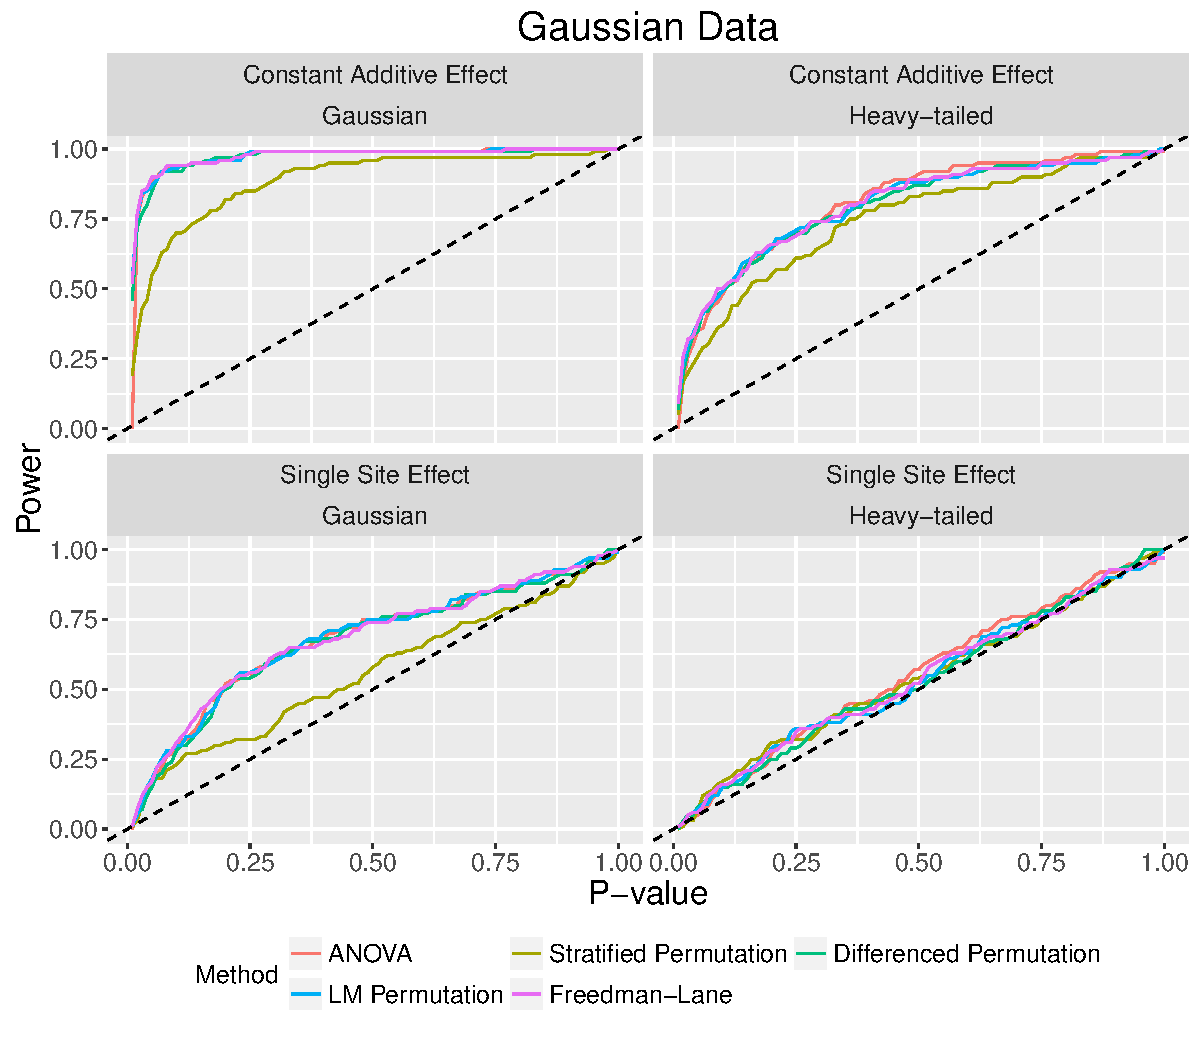
\includegraphics[width = \textwidth]{fig/normal_simulation_power.pdf}
\caption{Empirical power curves for the Gaussian simulated data}
\label{fig:normal_sim_power}
\end{figure}
%\begin{center}
%\begin{table}[ht]
\centering
\begin{tabular}{p{1.15in}|p{0.7in}|p{0.6in}p{0.8in}p{0.8in}p{0.8in}p{0.75in}}
  \hline
Treatment & Errors & ANOVA & Stratified Permutation & Differenced Permutation & LM Permutation & Freedman-Lane \\ 
  \hline
Constant Additive Effect & Gaussian & 0.89 & 0.55 & 0.86 & 0.89 & 0.89 \\ 
  Single Stratum Effect & Gaussian & 0.16 & 0.09 & 0.16 & 0.16 & 0.17 \\ 
  Constant Additive Effect & Heavy-tailed & 0.35 & 0.24 & 0.38 & 0.40 & 0.39 \\ 
  Single Stratum Effect & Heavy-tailed & 0.07 & 0.08 & 0.08 & 0.08 & 0.08 \\ 
   \hline
\end{tabular}
\caption{Empirical power at level $0.05$ for Gaussian simulated data} 
\label{tab:normal_power}
\end{table}

%\end{center}



\begin{table}[]
\centering
\label{tab:normal_power}
\begin{tabular}{ll|ccccc}
\multicolumn{2}{c|}{Design}                                                                  & \multicolumn{5}{c}{$p$-value}                                                                                                                                                                                                                                                                                                                                           \\ \hline
Errors                        & \begin{tabular}[c]{@{}l@{}}Treatment \\ Effect\end{tabular} & \multicolumn{1}{l}{ANCOVA} & \multicolumn{1}{l}{\begin{tabular}[c]{@{}l@{}}Stratified\\ Permutation\end{tabular}} & \multicolumn{1}{l}{\begin{tabular}[c]{@{}l@{}}Differenced\\ Permutation\end{tabular}} & \multicolumn{1}{l}{\begin{tabular}[c]{@{}l@{}}LM\\ Permutation\end{tabular}} & \multicolumn{1}{l}{\begin{tabular}[c]{@{}l@{}}Freedman-\\ Lane\end{tabular}} \\ \hline
\multirow{3}{*}{Gaussian}     & None                                                        & 0.058                      & 0.042                                                                                & 0.038                                                                                 & 0.062                                                                        & 0.057                                                                        \\
                              & Constant                                                    & 0.886                      & 0.545                                                                                 & 0.858                                                                                 & 0.891                                                                        & 0.892                                                                        \\
                              & Single stratum                                              & 0.159                      & 0.089                                                                                & 0.160                                                                                 & 0.162                                                                        & 0.170                                                                        \\ \hline
\multirow{3}{*}{Heavy-tailed} & None                                                        & 0.032                      & 0.040                                                                                & 0.045                                                                                 & 0.042                                                                        & 0.040                                                                        \\
                              & Constant                                                    & 0.355                      & 0.240                                                                                & 0.378                                                                                 & 0.400                                                                        & 0.393                                                                        \\
                              & Single stratum                                              & 0.066                      & 0.080                                                                                & 0.082                                                                                 & 0.076                                                                        & 0.080                                                                        \\ \hline
\end{tabular}
\caption{Empirical power at level $0.05$ for Gaussian simulated data.}
\end{table}

Our second set of simulations used the same design as the previous ones, but modified the sizes of the treatment groups.
Within each stratum, 4 individuals received one treatment and 12 received the other.
This mimics real-world experiments, where the more expensive treatment is administered less frequently than the other.
It is well-known that both parametric and nonparametric tests have higher than nominal level when there is heterogeneous variance, and this effect is exacerbated when group sizes are unequal (\cite{glass_consequences_1972}, \cite{zimmerman_two_2006}).
Here, the data have the same variance so we would expect power, not the test level, to be an issue.
(See the supplementary Gaussian simulations for a discussion of heterogeneous variances.)
We omit a plot of the power curves from these simulations, as the patterns appear similar to those in Figure~\ref{fig:normal_sim_power}.
Table~\ref{tab:imbalanced_power} displays the value of these power curves and the size of the test at level $0.05$.
In this case, the permutation tests (except for the simple stratified permutation) have slightly higher power than the ANCOVA, but the difference is not substantial.
%\begin{figure}
%\centering
%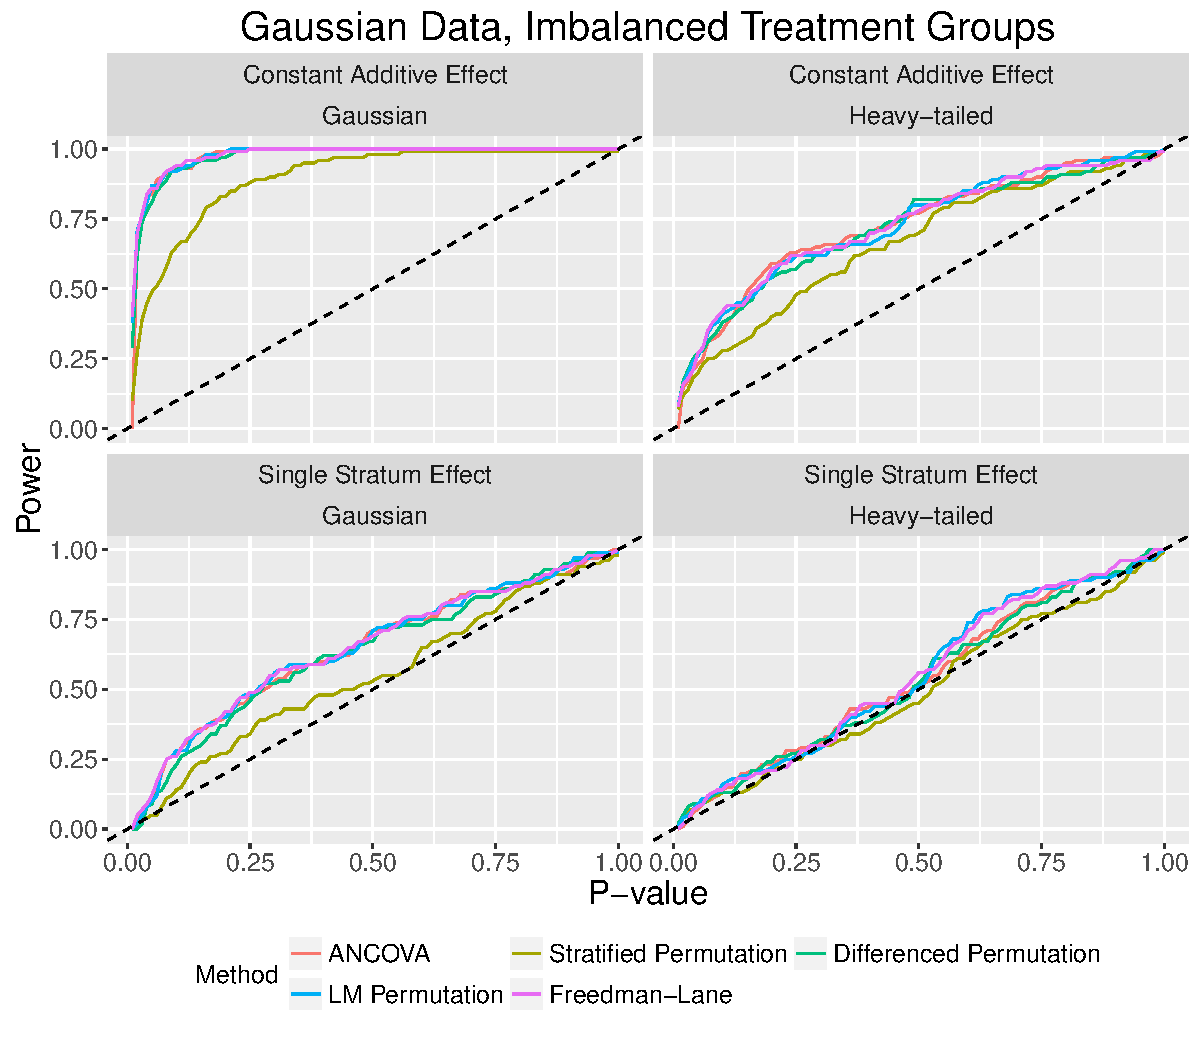
\includegraphics[width = \textwidth]{fig/imbalanced_simulation_power}
%\caption{Empirical power curves for the Gaussian simulated data with imbalanced group sizes}
%\label{fig:imbalanced_sim_power}
%\end{figure}
%\begin{center}
%\begin{table}[ht]
\centering
\begin{tabular}{|p{0.7in}|p{0.6in}p{0.8in}p{0.8in}p{0.8in}p{0.8in}p{0.75in}}
  \hline
Treatment & Errors & ANCOVA & Stratified Permutation & Differenced Permutation & LM Permutation & Freedman-Lane \\ 
  \hline
No Effect & Gaussian & 0.046 & 0.031 & 0.028 & 0.042 & 0.045 \\ 
  Constant Additive Effect & Gaussian & 0.840 & 0.490 & 0.810 & 0.870 & 0.860 \\ 
  Single Stratum Effect & Gaussian & 0.120 & 0.050 & 0.090 & 0.100 & 0.120 \\ 
   \hline
No Effect & Heavy-tailed & 0.034 & 0.054 & 0.055 & 0.047 & 0.042 \\ 
  Constant Additive Effect & Heavy-tailed & 0.230 & 0.200 & 0.270 & 0.260 & 0.270 \\ 
  Single Stratum Effect & Heavy-tailed & 0.070 & 0.080 & 0.090 & 0.090 & 0.080 \\ 
   \hline
\end{tabular}
\caption{Empirical power at level $0.05$ for Gaussian simulated data with imbalanced treatment groups} 
\label{tab:imbalanced_power}
\end{table}

%\end{center}


\begin{table}[ht]
\centering
\label{tab:imbalanced_power}
\begin{tabular}{ll|ccccc}
\multicolumn{2}{c|}{Design}                                                                 & \multicolumn{5}{c}{$p$-value}                                                                                                                                                                                                                                                                                                                                           \\ \hline
Errors                        & \begin{tabular}[c]{@{}l@{}}Treatment \\ Effect\end{tabular} & \multicolumn{1}{l}{ANCOVA} & \multicolumn{1}{l}{\begin{tabular}[c]{@{}l@{}}Stratified\\ Permutation\end{tabular}} & \multicolumn{1}{l}{\begin{tabular}[c]{@{}l@{}}Differenced\\ Permutation\end{tabular}} & \multicolumn{1}{l}{\begin{tabular}[c]{@{}l@{}}LM\\ Permutation\end{tabular}} & \multicolumn{1}{l}{\begin{tabular}[c]{@{}l@{}}Freedman-\\ Lane\end{tabular}} \\ \hline
\multirow{3}{*}{Gaussian}     & None                                                        & 0.046                      & 0.031                                                                                & 0.028                                                                                 & 0.042                                                                        & 0.045                                                                        \\
                              & Constant                                                    & 0.840                      & 0.490                                                                                & 0.810                                                                                 & 0.870                                                                        & 0.860                                                                        \\
                              & Single stratum                                              & 0.120                      & 0.050                                                                                & 0.090                                                                                 & 0.100                                                                        & 0.120                                                                        \\ \hline
\multirow{3}{*}{Heavy-tailed} & None                                                        & 0.034                      & 0.054                                                                                & 0.055                                                                                 & 0.047                                                                        & 0.042                                                                        \\
                              & Constant                                                    & 0.230                      & 0.200                                                                                & 0.270                                                                                 & 0.260                                                                        & 0.270                                                                        \\
                              & Single stratum                                              & 0.070                      & 0.080                                                                                & 0.090                                                                                 & 0.090                                                                        & 0.080                                                                        \\ \hline
\end{tabular}
\caption{Empirical power at level $0.05$ for Gaussian simulated data with imbalanced treatment groups} 
\end{table}

In our third set of simulations, we made the baseline measurements $Y_{ij0}$ discrete and skewed.
This type of data occurs in some surveys where individuals are asked to rate their symptom severity or some experience on a scale from 1 to 10, for instance.
We generated the baseline measures using independent draws from a Poisson distribution with mean 4 and censored values at 10.
We conditioned on these observed baseline measures after we having generated them once.
Then, for each 1000 trials, we randomly assigned treatment to half of the individuals in each stratum and generated errors taking on values $0.5$ and $-0.5$ with equal probability.
We constructed $Y_{ij1}$ using Equation~\ref{eqn:dgp} with a treatment effect of $\gamma = 0.5$.
However, we didn't observe $Y_{ij1}$ but instead integer values $\tilde{Y}_{ij1}$ defined as 

\begin{displaymath}
   \tilde{Y}_{ij1} = \left\{
     \begin{array}{ll}
       1 & \text{if } \tilde{Y}_{ij1} < 1\\
       10 & \text{if } \tilde{Y}_{ij1} > 10 \\
       \lfloor \tilde{Y}_{ij1} \rfloor & \text{otherwise}
     \end{array}
   \right.
\end{displaymath}

The observed outcomes $\tilde{Y}_{ij1}$, the baseline measures $Y_{ij0}$, and the errors are discrete.
The normality assumption is clearly violated here.

We examined the effect of stratum size in this set of simulations.
For each of the two treatment effect designs, we considered both equal and unequal stratum sizes.
First, we considered balanced samples as before, where each stratum contained $n_j = 16$ individuals.
Next, we considered imbalanced strata, where the smallest stratum had only $n_1=8$ individuals, the next had $n_2= 16$, and the largest had $n_3=24$.
The design with a single stratum effect and unequal stratum sizes was particularly unfavorable for hypothesis testing:
the nonzero effect only occured in the smallest stratum.

Figure~\ref{fig:skewed_sim_power} shows the estimated power curves in these four designs.
When the treatment effect is constant, sample sizes within each stratum don't matter; 
the two power curve plots in the first row of Figure~\ref{fig:skewed_sim_power} look the same up to chance variation.
When the treatment effect only occurs in one stratum, there is a substantial loss in power.
It is nearly impossible to detect a difference in treatments when the affected stratum is too small.
In practice, one does not usually know a priori which individuals will be affected by treatment (otherwise, those not affected would be excluded from the study altogether).
This result suggests that when stratifying, one must be cautious not to stratify too finely, otherwise treatment effects may be indistinguishable from random variability.

All of the tests appear to be conservative and have lower than nominal level.
As in the first set of simulations, the stratified permutation test using the raw outcomes has the lowest power of the five tests.
Now, however, the stratified permutation test using the change scores also has lower power than the three linear model tests.
Presumably, this is because the differences $\tilde{Y}_{ij1} - Y_{ij0}$ are discrete and lie in a small range of values, so the test statistic does not vary greatly across permutations.
Table~\ref{tab:skewed_power} confirms this: power for the three linear model methods is high when the treatment is constant across strata, and power for all of the methods suffers when the effect is isolated in a single stratum.


\begin{figure}
\centering
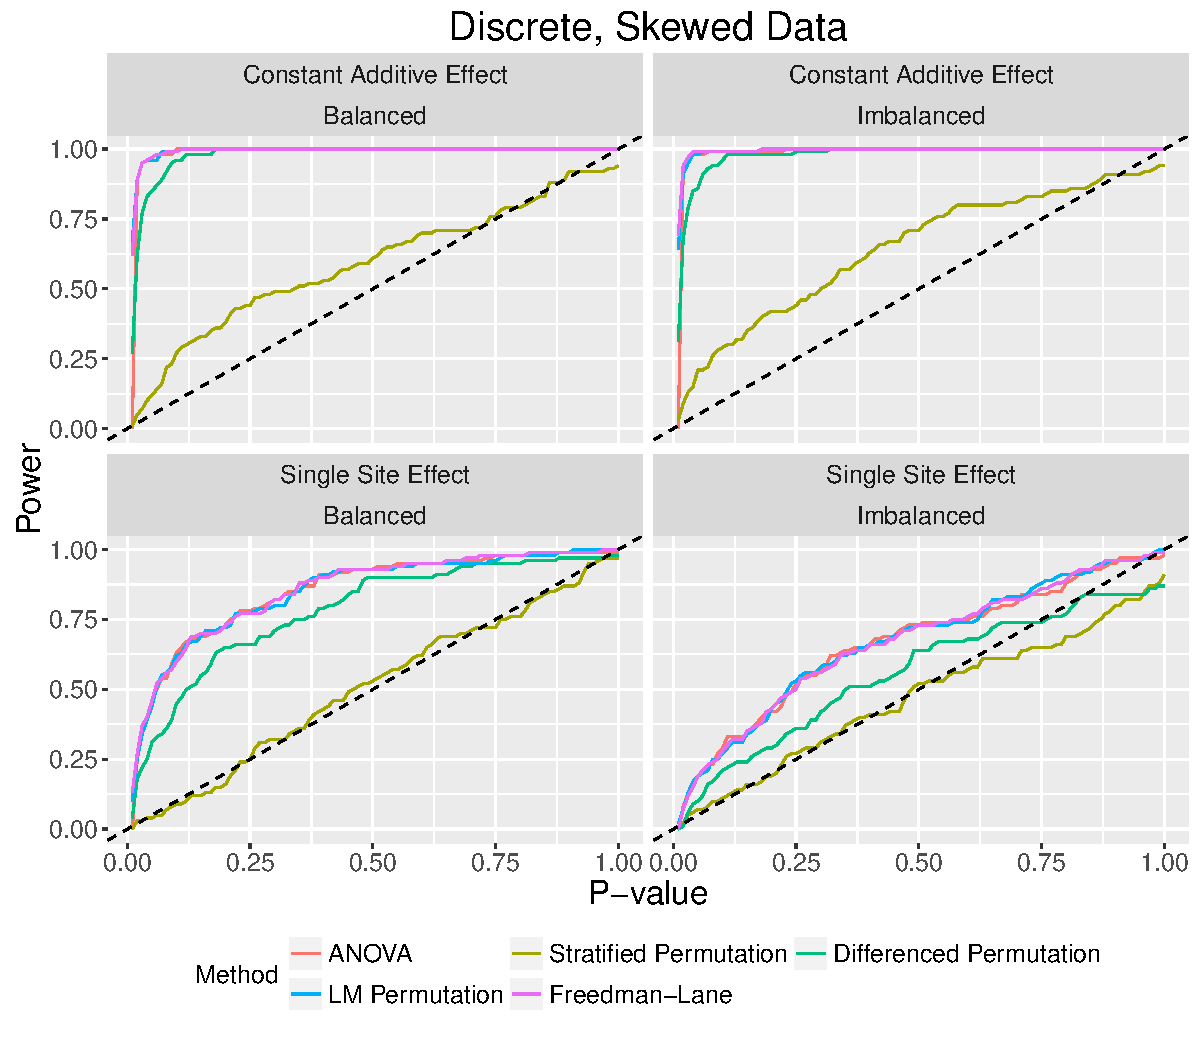
\includegraphics[width = \textwidth]{fig/skewed_simulation_power.pdf}
\caption{Empirical power curves for the skewed, discrete simulated data}
\label{fig:skewed_sim_power}
\end{figure}

%\begin{center}
%\begin{table}[ht]
\centering
\begin{tabular}{p{1.25in}|p{0.7in}|p{0.6in}p{0.8in}p{0.8in}p{0.8in}p{0.75in}}
  \hline
Treatment & Design & ANCOVA & Stratified Permutation & Differenced Permutation & LM Permutation & Freedman-Lane \\ 
  \hline
No Effect & Balanced & 0.036 & 0.025 & 0.021 & 0.035 & 0.037 \\ 
  Constant Additive Effect & Balanced & 0.974 & 0.143 & 0.853 & 0.972 & 0.977 \\ 
  Single Stratum Effect & Balanced & 0.422 & 0.050 & 0.275 & 0.429 & 0.424 \\ 
   \hline
No Effect & Imbalanced & 0.038 & 0.024 & 0.019 & 0.037 & 0.039 \\ 
  Constant Additive Effect & Imbalanced & 0.971 & 0.147 & 0.860 & 0.970 & 0.972 \\ 
  Single Stratum Effect & Imbalanced & 0.190 & 0.070 & 0.100 & 0.190 & 0.190 \\ 
   \hline
\end{tabular}
\caption{Empirical power at level $0.05$ for discrete, skewed simulated data} 
\label{tab:skewed_power}
\end{table}

%\end{center}
\begin{table}[]
\centering
\label{tab:skewed_power}
\begin{tabular}{ll|ccccc}
\multicolumn{2}{c|}{Design}                                                               & \multicolumn{5}{c}{$p$-value}                                                                                                                                                                                                                                                                                                                                           \\ \hline
Group sizes                 & \begin{tabular}[c]{@{}l@{}}Treatment \\ Effect\end{tabular} & \multicolumn{1}{l}{ANCOVA} & \multicolumn{1}{l}{\begin{tabular}[c]{@{}l@{}}Stratified\\ Permutation\end{tabular}} & \multicolumn{1}{l}{\begin{tabular}[c]{@{}l@{}}Differenced\\ Permutation\end{tabular}} & \multicolumn{1}{l}{\begin{tabular}[c]{@{}l@{}}LM\\ Permutation\end{tabular}} & \multicolumn{1}{l}{\begin{tabular}[c]{@{}l@{}}Freedman-\\ Lane\end{tabular}} \\ \hline
\multirow{3}{*}{Balanced}   & None                                                        & 0.036                      & 0.025                                                                                & 0.021                                                                                 & 0.035                                                                        & 0.037                                                                        \\
                            & Constant                                                    & 0.974                      & 0.143                                                                                & 0.853                                                                                 & 0.972                                                                        & 0.977                                                                        \\
                            & Single stratum                                              & 0.422                      & 0.050                                                                                & 0.275                                                                                 & 0.429                                                                        & 0.424                                                                        \\ \hline
\multirow{3}{*}{Imbalanced} & None                                                        & 0.038                      & 0.024                                                                                & 0.019                                                                                 & 0.037                                                                        & 0.039                                                                        \\
                            & Constant                                                    & 0.971                      & 0.147                                                                                & 0.860                                                                                 & 0.970                                                                        & 0.972                                                                        \\
                            & Single stratum                                              & 0.190                      & 0.070                                                                                & 0.100                                                                                 & 0.190                                                                        & 0.190                                                                        \\ \hline
\end{tabular}
\caption{Empirical power at level $0.05$ for discrete, skewed simulated data} 
\end{table}
It makes sense that in all of these simulations, the permutation test using the change scores as the response measure is more powerful than the permutation test using the raw outcomes.
The baseline and outcome are highly correlated, so the change score has lower variance the outcome alone.
In additional simulations, 
we modified the data-generating process given by Equation~\ref{eqn:dgp} so that the outcome and baseline had correlation of $0.25$ (see the supplementary Gaussian simulations for a more detailed treatment).
In this case, the result was reversed: 
the differenced test had low power while the test using the raw outcomes had a power curve closer to the linear model-based tests.
This behavior has been studied before by \cite{frison_repeated_1992}, who recommended to use the difference in outcome and baseline if their correlation is greater than $0.5$ and to use the outcome only if their correlation is less than $0.5$.



\subsection{Clinical data results}
We compared the parametric ANCOVA, the stratified permutation test, and the two linear model-based permutation tests using a dataset from a clinical trial comparing the effectiveness of two treatments for gastroesophageal reflux disease (GERD).
Patients were treated at eight sites in two different countries.
At each site, patients were randomly assigned one of two treatments.
Patients were observed for a week before receiving treatment and for a week after receiving treatment.
On each of the fourteen days of observation, patients responded to a survey about their heartburn, regurgitation, and dyspepsia frequency and severity.
These endpoints were measured on a discrete scale.
There were several additional endpoints, such as daily regurgitation, daily ``hrdq'', and daily dyspepsia, calculated from the survey measures.
Daily ``hrdq'' was the primary endpoint.
To reduce day-to-day variation, we averaged the measures from each week to obtain two time points per patient, one pretreatment and one post-treatment.

We treated site as the stratification variable, as this is the level at which treatment was randomized.
We did not include country in the model, as a country-level effect should be captured in the site-level effects.
The model used for the linear regression-based tests was defined as in Equation~\ref{eqn:ancova}.
This model allowed for the intercept $\alpha_j$ to vary across sites and used the pretreatment, baseline measurement as the control variable $\mathbf{X}$.
The outcome and baseline had a low correlation (for instance, $0.56$ for daily ``hrdq''), so we used raw outcomes and not the change scores as the dependent variable. 
As our simulations and previous work \cite{frison_repeated_1992} show, when the correlation between baseline and outcome is low, it is more powerful to control for baseline outcomes using a model.

Figure~\ref{fig:clinical_distr} shows the distribution of each clinical endpoint for the two treatment groups.
There is a clear difference in distributions for daily heartburn (``daily\_heart''), daily ``hrdq'', and heartburn frequency (``heart\_freq'').
The difference is less clear for daily regurgitation (``daily\_regurg'') and regurgitation frequency (``regurg\_freq'').

Table~\ref{tab:clinical_pvalues} shows the $p$-values for the four tests.
Overall, the results confirm our expectations based on visual comparison in Figure~\ref{fig:clinical_distr}:
one or more of the tests reject the null hypothesis that outcomes are the same between treatments for heartburn frequency, daily heartburn, and daily ``hrdq,''
but not for any of the other endpoints.
The three tests based on the linear model all give similar results here.
The $p$-values for the ANCOVA tend to be smaller than the linear model and the residual permutation tests, while the $p$-values stratified, unadjusted permutation test have no consistent pattern.
The parametric test has comparable or slightly higher power than the other permutation tests.

\begin{figure}
\centering
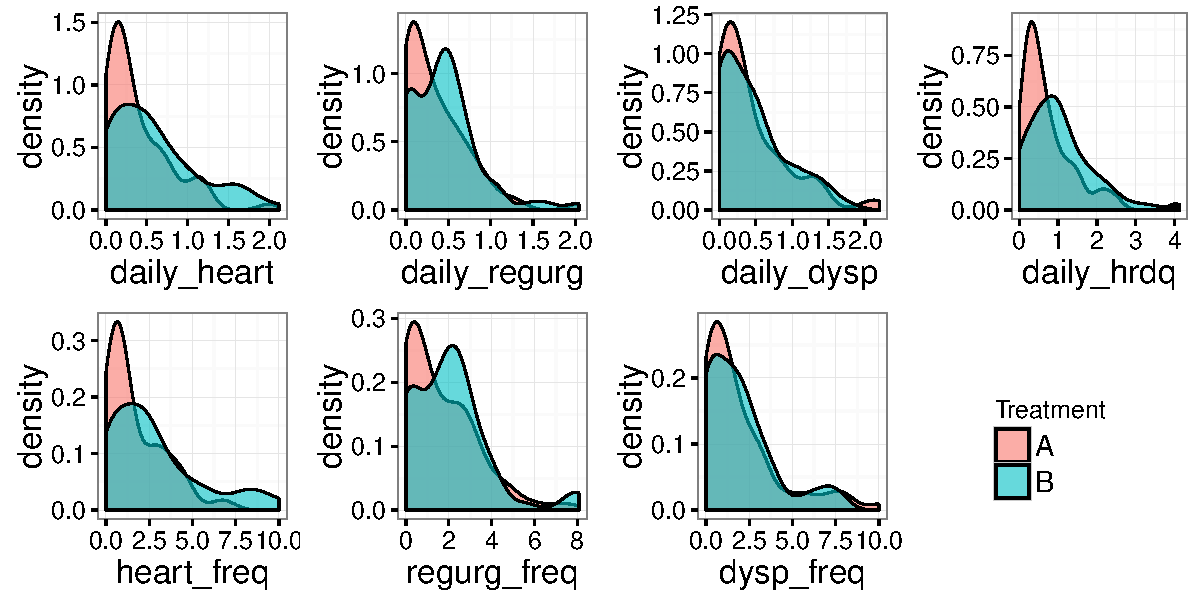
\includegraphics[width = \textwidth]{fig/clinical_distr.pdf}
\caption{Distribution of each endpoint for the two treatments A and B}
\label{fig:clinical_distr}
\end{figure}

%
%\begin{center}
%\begin{table}[ht]
\centering
\begin{tabular}{r|p{1.2in}p{1.2in}p{1.2in}p{1.2in}}
  \hline
 & Parametric ANCOVA & Stratified permutation & LM permutation & Residual permutation \\ 
  \hline
heart\_freq & 0.035 & 0.006 & 0.080 & 0.082 \\ 
  regurg\_freq & 0.136 & 0.118 & 0.280 & 0.220 \\ 
  dysp\_freq & 0.565 & 0.948 & 0.616 & 0.592 \\ 
  daily\_heart & 0.032 & 0.004 & 0.056 & 0.068 \\ 
  daily\_regurg & 0.142 & 0.174 & 0.286 & 0.246 \\ 
  daily\_hrdq & 0.043 & 0.012 & 0.088 & 0.098 \\ 
  daily\_dysp & 0.582 & 0.810 & 0.756 & 0.722 \\ 
   \hline
\end{tabular}
\caption{Comparison of p-values from four tests, for each continuous endpoint.} 
\label{tab:clinical_pvalues}
\end{table}

%\end{center}

\begin{table}[]
\centering
\label{tab:clinical_pvalues}
\begin{tabular}{l|cccc}
Endpoint      & \multicolumn{1}{l}{ANCOVA} & \multicolumn{1}{l}{\begin{tabular}[c]{@{}l@{}}Stratified\\ Permutation\end{tabular}} & \multicolumn{1}{l}{\begin{tabular}[c]{@{}l@{}}LM\\ Permutation\end{tabular}} & \multicolumn{1}{l}{\begin{tabular}[c]{@{}l@{}}Freedman-\\ Lane\end{tabular}} \\ \hline
heart\_freq   & 0.035                      & 0.006                                                                                & 0.080                                                                        & 0.082                                                                        \\
regurg\_freq  & 0.136                      & 0.118                                                                                & 0.280                                                                        & 0.220                                                                        \\
dysp\_freq    & 0.565                      & 0.948                                                                                & 0.616                                                                        & 0.592                                                                        \\
daily\_heart & 0.032                      & 0.004                                                                                & 0.056                                                                        & 0.068                                                                        \\
daily\_regur  & 0.142                      & 0.174                                                                                & 0.286                                                                        & 0.246                                                                        \\
daily\_hrdq   & 0.043                      & 0.012                                                                                & 0.088                                                                        & 0.098                                                                        \\
daily\_dysp   & 0.582                      & 0.810                                                                                & 0.756                                                                        & 0.722                                                                        \\
\hline
\end{tabular}
\caption{Comparison of p-values from four tests, for each continuous endpoint.} 
\end{table}

\section{Discussion}
% This section should discuss the implications of the findings in context of existing research and highlight limitations of the study.

This paper adds to the literature comparing parametric and nonparametric tests.
Our results match those of \cite{vickers_parametric_2005, anderson_empirical_1999}, where parametric ANCOVA and regression-based $t$ tests performed the same or better than the comparable nonparametric tests.
We simulated a variety of data-generating processes ranging from the ideal case when all assumptions are met 
to the case when data are non-normal, discrete, or skewed,
as well as data with other possible issues such as heterogeneous treatment effects and imbalanced sample sizes.
When the ANCOVA assumptions were violated, the linear regression-based tests lost power relative to the best case data-generating process where all assumptions were satisfied.
However, the power of the tests remained the same \textit{relative to each other}.
It is a matter of taste which test one chooses for their experiment: while the parametric test may be robust to violations of its assumptions, it is somewhat reassuring that the permutation test can exactly match the randomization that was done while making no distributional assumptions.

Permutation tests do not come entirely free of assumptions, though.  
\cite{romano_behavior_1990} warns against using permutation tests naively if items are not truly exchangeable. 
For instance, he points to the case where observations have unequal variances.  
This is a problem as we cannot observe the errors; it is a leap of faith to assert that they are homogeneous and therefore exchangeable.
\cite{boik_fisherpitman_1987} illustrates this phenomenon using the normal theory $F$ test and its permutation counterpart, 
and demonstrates by simulation that the latter has larger than nominal level when the error variances are heterogeneous.

It is important to note that the permutation tests described here are approximately exact only in the context of randomized experiments.
In this case, treatment is assigned at random and is therefore statistically independent of the covariates $\mathbf{X}$ and the errors $\mathbf{\varepsilon}$.
Conversely, in observational studies, treatment may be associated with $\mathbf{X}$ and/or $\mathbf{\varepsilon}$, often in a way that is difficult or impossible to model.
Independence, or the weaker condition of exchangeability, is what enables us to construct permutation distributions while holding $\mathbf{X}$ fixed.
When exchangeability doesn't hold, we cannot disentangle the effect of $\mathbf{Z}$ from the effect of $\mathbf{X}$.
One must provide evidence that items in observational studies are exchangeable in order to achieve an approximately exact test.
The onus is on the researcher to make the case that the object being permuted is uncorrelated with the other variables being held fixed.
This can be done visually using scatterplots and residual plots \cite{freedman_nonstochastic_1983} and from subject-matter knowledge.

One should be mindful of which covariates to control for.
Ideally, one knows and observes all covariates related to the outcome.
In that case, the coefficient for treatment in a fully saturated linear model (including all covariates and their interactions) is an asymptotically consistent estimate of the average treatment effect \cite{lin_agnostic_2013}.
It is rare that one knows \textit{all} relevant covariates in practice; failure to control for all relevant variables can introduce bias in certain permutation tests.
 \cite{gail_tests_1988} propose a randomization test based on residuals from an exponential family model and find that omitting relevant covariates leads to tests with higher than nominal level.
 
The method of controlling for baseline covariates matters, too.
The naive way is to consider change scores, subtracting baseline measures from the outcome and doing hypothesis testing using the change as the dependent variable.
Our simulations confirm the suggestion of \cite{frison_repeated_1992} to use change scores only when there is a strong correlation between baseline and outcome.
Weak correlations between baseline and outcome occur often in practice, as was the case with our GERD dataset.
If the correlation is weak, then the resulting test using the difference may be less powerful than ignoring the baseline altogether.
Instead, we suggest incorporating the baseline in a regression model.
This is more general than using differences;
treating the change scores as the dependent variable is a special case of the linear regression, constraining the coefficient on the baseline measure to be $1$.
The regression approach is more flexible and demonstrably more powerful.



\bigskip
\begin{center}
{\large\bf SUPPLEMENTARY MATERIAL}
\end{center}

\begin{description}

\item[Title:] Brief description. (file type)

\end{description}

\bibliographystyle{chicago}

\bibliography{references}
\end{document}
